\documentclass{standalone}
\usepackage{tikz}
\usetikzlibrary{automata, positioning}

\begin{document}
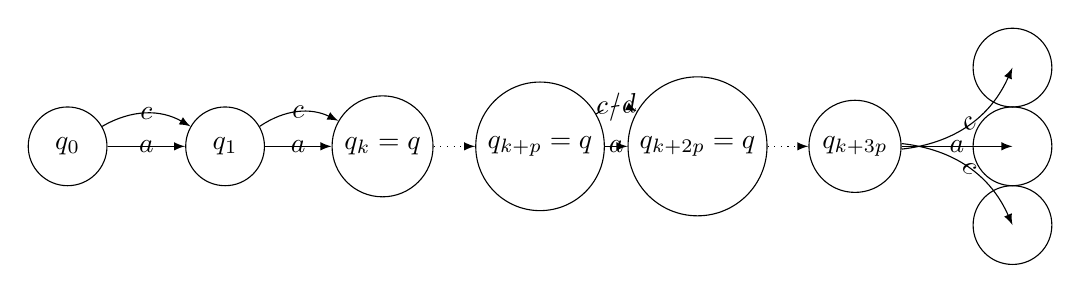
\begin{tikzpicture}[
    ->,
    >=latex,
    node distance=2cm and 2cm,
    on grid,
    initial text=,
    state/.style={circle, draw, minimum size=1cm},
    path label/.style={midway, anchor=center, sloped}
]

% Define nodes
\node[state] (q0) at (0,0) {$q_0$};
\node[state] (q1) at (2,0) {$q_1$};
\node[state] (qk) at (4,0) {$q_k=q$};
\node[state] (qkp) at (6,0) {$q_{k+p}=q$};
\node[state] (qk2p) at (8,0) {$q_{k+2p}=q$};
\node[state] (qk3p) at (10,0) {$q_{k+3p}$};

% Draw edges with labels
\draw (q0) -- node[path label] {$a$} (q1);
\draw (q0) to[bend left] node[path label] {$c$} (q1);

\draw (q1) -- node[path label] {$a$} (qk);
\draw (q1) to[bend left] node[path label] {$c$} (qk);

\draw[dotted] (qk) -- (qkp);

\draw (qkp) -- node[path label] {$a$} (qk2p);
\draw[dashed] (qkp) to[bend left] node[path label] {$c/d$} (qk2p);

\draw[dotted] (qk2p) -- (qk3p);

\draw (qk3p) to[bend left] node[path label] {$c$} ++(2,-1) node[state] {};
\draw (qk3p) -- node[path label] {$a$} ++(2,0) node[state] {};
\draw (qk3p) to[bend right] node[path label] {$c$} ++(2,1) node[state] {};

\end{tikzpicture}
\end{document}